\subsection*{Kategorisering}
Kategoriseringsfunktionen inddeles i tre klasser af typen boundary og en dertilhørende controller, som det fremgår af \autoref{fig:DesignKategorisering}.

\begin{figure} [H]
\centering
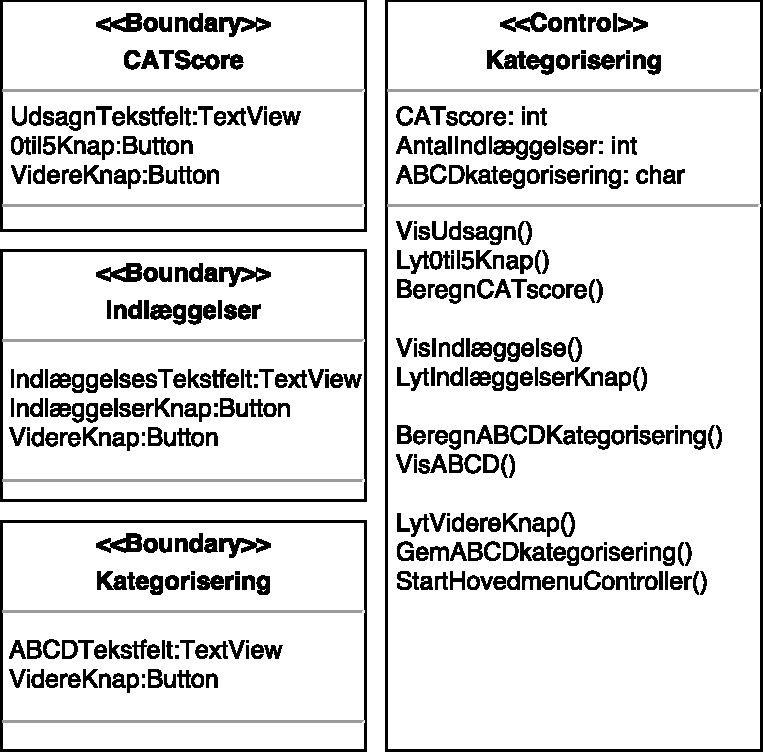
\includegraphics[width=0.9\textwidth]{figures/MVC/MVCKategorisering}
\caption{Designklasser for kategorisering.}
\label{fig:DesignKategorisering}
\end{figure}

\noindent
Kategoriseringen inddeles i tre grænseflader, herunder \textit{CATScore}, \textit{Indlæggelser} samt \textit{Kategorisering}. Dette er valgt, da det ønskes at gøre app’en overskuelig samt
brugervenlig. Hertil skal brugeren foretage minimale valg på hver brugergrænseflade, således
brugeren ikke eksponeres til for mange valg samt informationer. De tre grænseflader indeholder tekstfelter, der informerer brugeren om den følgende handling. Dertil er der ligeledes opsat knapper af typen button, således brugeren kan besvare spørgsmålene. 

Controlleren, \textit{Kategorisering}, håndterer visningen af de tre boundarys samt respektive knapper og tekst. Der er ligeledes udarbejdet et sekvensdiagram for kategorisering, hvilket ses af \autoref{fig:SEKKategorisering}.

\begin{figure} [H]
\centering
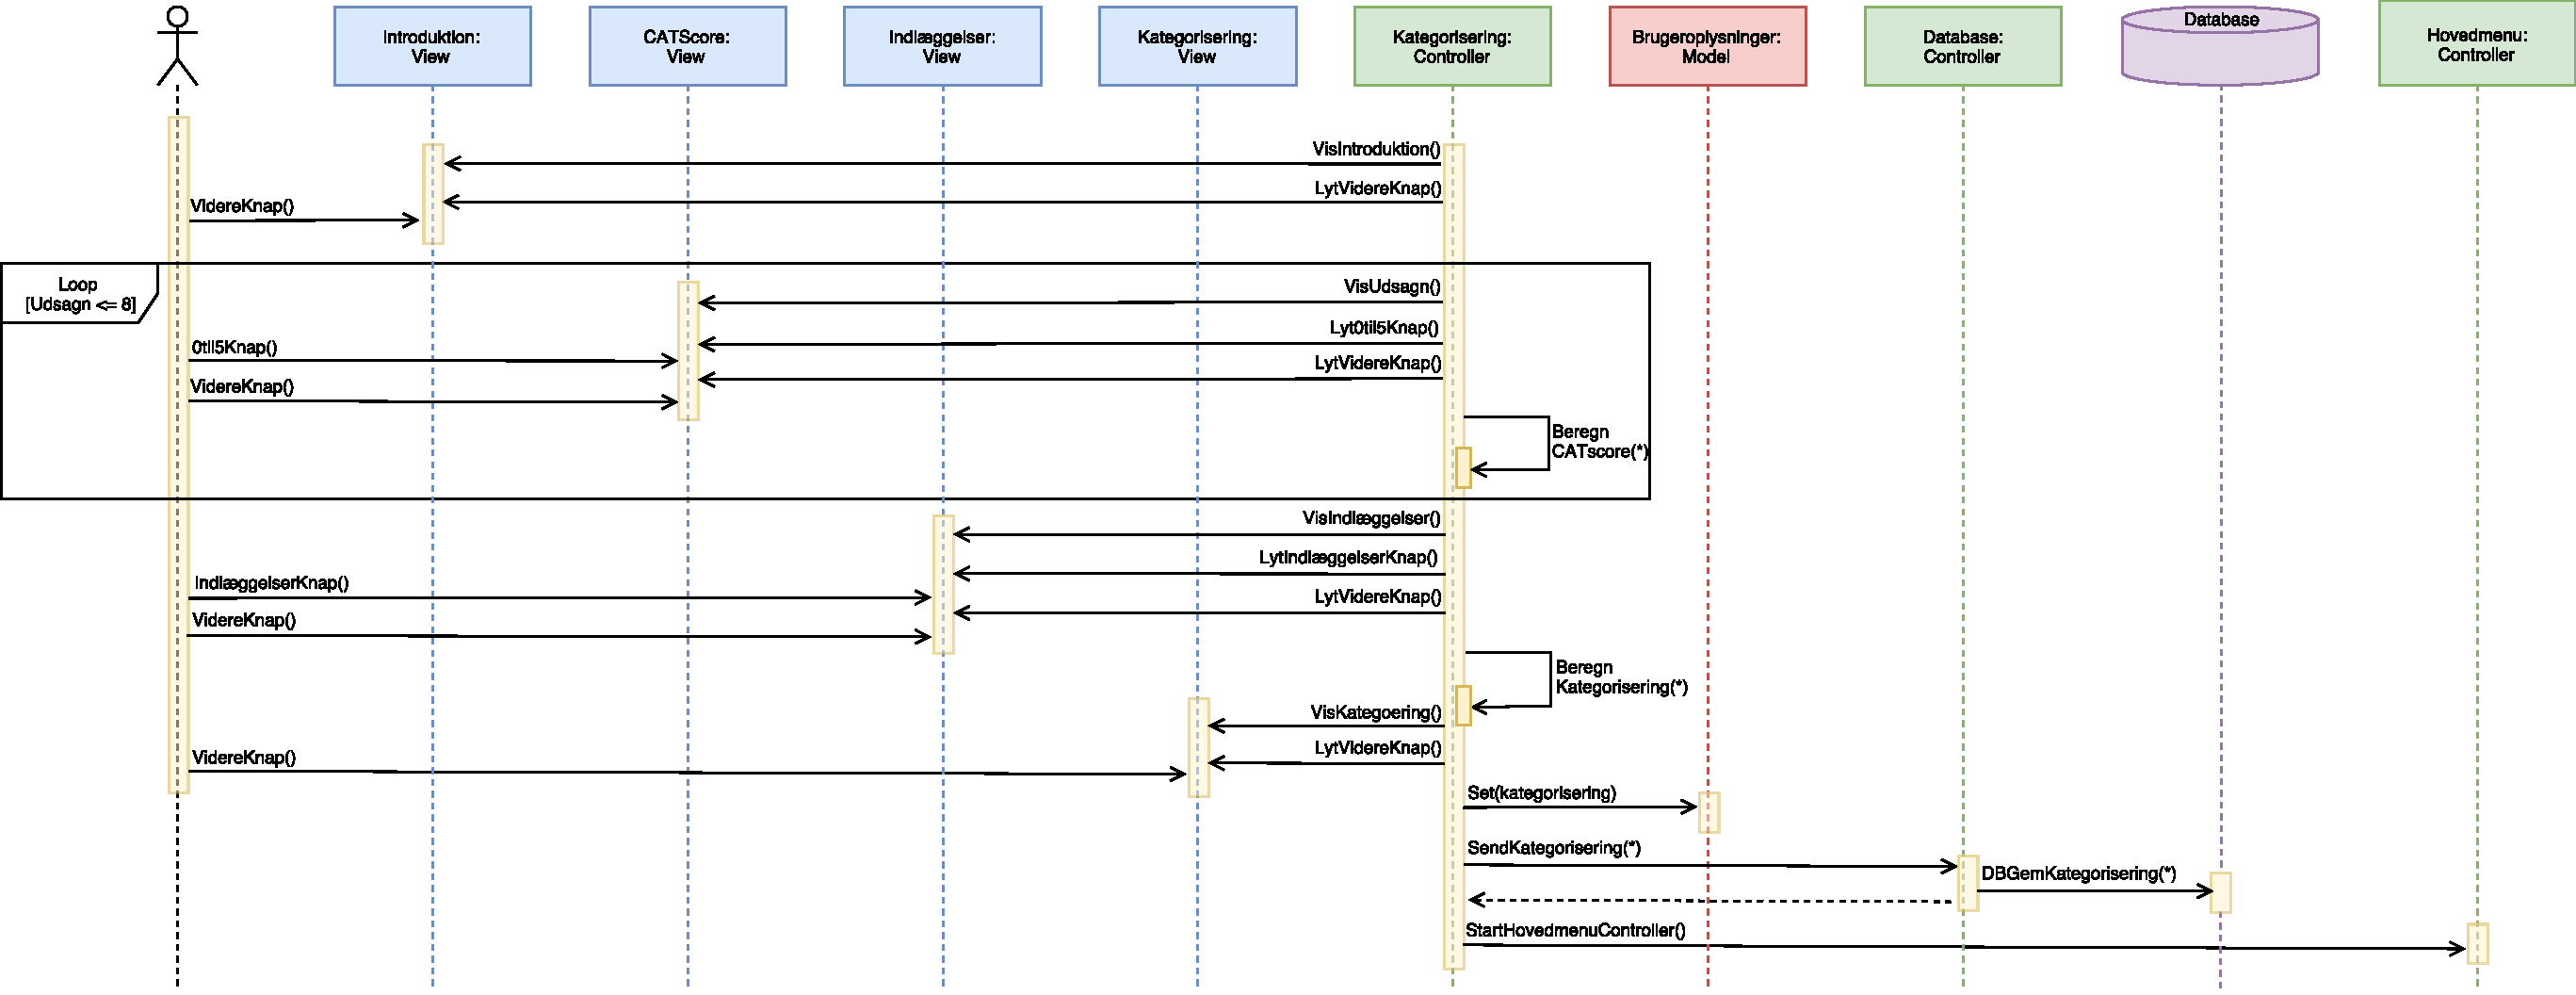
\includegraphics[width=1\textwidth]{figures/Sek/SEKKategorisering}
\caption{Sekvensdiagram for kategorisering.}
\label{fig:SEKKategorisering}
\end{figure}

Det fremgår af sekvensdiagrammet, at grænsefladen for \textit{CATScore} vises som det første. Hertil er der opstillet en loop, som har til formål at stille otte spørgsmål som brugeren skal besvare ved hjælp af knapper, \textit{0til5Knap}. Idet brugeren trykker videre, adderes CAT-scoren. Efter de otte udsagn er besvaret og den samlet CAT-score er fundet, vises grænsefladen for \textit{Indlæggelser}. Controlleren lytter dertil til \textit{IndlæggelserKnap}, hvori brugeren besvarer antal årlige indlæggelser forårsaget af KOL. Besvarelsen bekræftes ved at benytte \textit{VidereKnappen}. ABCD-kategoriseringen kan derved beregnes og vises i \textit{Kategorisering} grænsefladen. Denne kategorisering gemmes i entityen \textit{Brugeroplysninger}, når brugeren trykker videre. Herefter startes hovedmenuen.
